% Chapter Template

\documentclass{report}
\usepackage{subfigure}
\usepackage{comment}
\usepackage{graphicx}
%\graphicspath{ {Pictures/} }
\begin{document}
\chapter{Intoduction} % Main chapter title

%\label{Chaptery 1} % Change X to a consecutive number; for referencing this chapter elsewhere, use \ref{ChapterX}

%\lhead{Chapter 1. \emph{Sample}} % Change X to a consecutive number; this is for the header on each page - perhaps a shortened title

%----------------------------------------------------------------------------------------
%	SECTION 1
%---------------------------------------------------------------------------------------
%\section{}





The advent of credit cards and their increasing functionality have not only given people more personal comfort, but have also attracted malicious characters interested in the handsome rewards to be earned. Credit cards are nice target for fraud, since in a very short time a lot of money can be earned without taking many risks. This is because often the crime is only discovered a few weeks after the date. Credit card fraud can be defined as “unauthorized account activity by a person for which the account was not intended. Operationally, this is an event for which action can be taken to stop the abuse in progress and incorporate risk management practices to protect against similar actions in the future”. In simple terms, credit card fraud is defined when an individual uses another individual’s credit card for personal benefit while the owner of the card and the card issuer are not aware of the fact that the card is being misused. And the person using the card has not at all having the connection with the card holder or the issuer and has no intention of making the repayments for the purchase they done. 
%\subsection{•}


%\section{Adding another section}
%You can show a lot of figures together like these 


%Tables can be added like this

\chapter{DIFFERENT TYPES OF FRAUD TECHNIQUES}

There are three classes of frauds namely card related, merchant related and internet frauds. Some of them are listed below

\section{Card Related Frauds}

\subsection{Lost/Stolen Card:}
 This type of fraud occurs when the fraudster simply steals a customer’s card. In this case, the customer might feel he has lost his card, but actually this card might have been acquired by an attacker. 

\subsection{Account Takeover:}
This type of fraud occurs when the valid customer’s personal information is taken by fraudsters. The fraudsters takes control of a legitimate account by either providing the customer’s account number or the card number. The fraudster then contacts the card issuer, as the genuine card holder, to ask the mail to redirect to a new address. The fraudster reports card lost and asks for a replacement to be sent. 

\subsection{Cardholder-Not-Present (CNP):}
CNP transactions are performed only on the internet that is remotely, in such kind of frauds neither the card nor the cardholder is present at the point-of-sale. This take many types of transactions such as orders made over the phone or Internet, by mail order or fax. In such transactions, retailers are unable to physically check user or identity of the card holder which makes the user unknown and able to disguise their true identity, The details of the credit card are normally copied without the cardholder’s knowledge, collected from the receipts thrown by the customer or obtained by skimming process. Frequently obtained card details are generally used with fabricated personal details to make fraudulent CNP purchases. This means that while the three or four digit card security code (CVV number) on the back of cards can help prevent fraud where card details have been obtained, but when the card is stolen it won’t be helpful.
 

\subsection{Erasing the Magnetic strip:}
This is the type of fraud where the fraudsters erase the magnetic stripe by using the powerful electromagnet. The fraudsters then tampers with the details on the card so that they match the details of a valid card, which they may have attained, for example, when the fraudster begins to use the card, the cashier will swipe the card through the terminal several times, before realizing that the metallic strip does not work. The cashier will then proceed to manually input the card details into the terminal. This kind of fraud is having high risk because the cashier will be looking at the card closely to read the numbers.

\subsection{Phishing:}
Phishing is a type of fraud designed to steal a person’s identity. It is usually committed via spam e-mail or pop-up windows. Phishing works by a malicious person sending lots of false emails. The emails looks like they have come from a website or company you trust, for example your bank. The message tells you to provide the company with your personal details including your payment card details. They can claim that the reason for this is a database crash or something like this. To make the email look even more authentic, the fraudster might put a link to a website that look exactly like the real one but in fact that is not the real one and that is the fake one. These copies are often called “Spoofed websites”. When you are on the spoofed site they can ask you for even more personal details that will be directly transmitted to the person who made that website.  

\section{Merchant Related Frauds}
\subsection{Merchant Collusion:}
This type is done when a merchant purposely passes on his customer’s personal information to fraudsters. 

\subsection{Triangulation:}
Here, the fraudster creates a fake website and operates from there. Many discounts are given to the customers through this website due to which users are attracted to such websites. They purchase items and there they enter their personal information. Then this information is obtained by the fraudsters and they use it to perform illegimitate transactions.  

\section{Internet Frauds}
\subsection{False Merchant Sites:}
 In this type, the website asks the customers to enter their personal details if they want to access the content of the website. In this way, these fraudsters collect many credit card number which they use later for performing fraudulent transactions.

\subsection{Keystroke Loggers:}
“Keystroke logger” is a spyware which infects a user’s computer unknown to him. This spyware tracks all the details typed by the user and gives this information to the fraudster who thus obtains all the personal details.

\subsection{Cell phone camera Scan:}
When a customer is paying his bills, a fraudster may be roaming somewhere near him. The customer may be under the assumption that the attacker is busy chatting on his phone, but actually he is taking digital image of the computer’s details such as card number, expiry date, etc. This type of fraud is possible because of powerful cameras used these days. 

\subsection{Site Cloning:}
Site cloning is where fraudsters close an entire site or just the pages from which the customer made a purchase. Customers have no reason to believe they are not dealing with the company that they wished to purchase goods or services from because the pages that they are viewing are identical to those of the real site. The cloned site will receive these details and send the customer a receipt of the transaction through the email just as the real company would do. The customer suspects nothing, while the fraudsters have all the details they need to commit credit card fraud.

\chapter{PROBLEMS WITH CREDIT CARD FRAUD DETECTION}

One of the biggest problems associated with fraud detection is the lack of both literature providing experimental results and of real world data for academic researchers to perform experiments on. This is because fraud detection is often associated with sensitive financial data that is kept confidential for reasons of customer privacy. 
\paragraph{}
We now enumerate some of the properties a fraud detection system should have in order to perform good results. 

\begin{itemize}
  \item The system should be able to handle skewed distributions, since only a very small percentage of all credit card transactions is fraudulent, To solve this problem, often the training sets are divided into pieces where the distribution is less skewed.

  \item The ability to handle noise. This is simply the presence of errors in the data, for instance incorrect dates. Noise in actual data limits the accuracy of generalization that can be achieved, no matter how extensive the training set is. One way to deal with this problem is by cleaning the data. 
  
  \item Overlapping data is another problem in this field. Many transactions may resemble fraudulent transactions, when actually they are legitimate. The opposite also happens, when a fraudulent transaction appears to be normal. 


\item The system should be able to adapt themselves to new kinds of fraud. Since after a while successful fraud techniques decrease in efficiency, due to the fact that they become well known. Then a “Good” fraud tries to find new and inventive ways of doing his job.

\item There is a need for good metrics to evaluate the classifier system. As an example, the overall accuracy is not suited for evaluation on a skewed distribution, since even with a very high accuracy, almost all fraudulent transactions can be misclassified. 


\end{itemize}

This means that there should be a decision layer on top of the fraud detection system. The decision layer decides what action to take when fraudulent behaviour is detected via the fraud detection system, taking into account factors like the amount of the transaction and the quality of the customer doing the transaction 

\chapter{ARTIFICIAL NEURAL NETWORKS}
\section{Definition}
Artificial Neural Network (ANN) is an efficient computing system whose central theme is borrowed from the analogy of biological neural networks. ANN acquires a large collection of units that are interconnected in some pattern to allow communication between the units. These units, referred to as nodes or neurons, are simple processors which operate in parallel.
Every neuron is connected with other neuron through a connection link. Each connection link is associated with a weight that has information about the input signal. This is the most useful information for neurons to solve a particular problem because the weight usually excites or inhibits the signal that is being communicated. Each neuron has an internal state, which is called an activation signal. Output signals, which are produced after combining the input signals and activation rule, may be sent to other units.



Neural Network exists in many ways and diffeent forms. The type of neural network we will discuss in this paper is the Feed Forward Multilayer Perceptron. A feedforward multilayer perceptron consists of different layers of perceptrons that are interconnected by a set of weighted connections We can distinguish three types of layers:

\subsection{Input}
Input layer Receives input from an input stream, which can be database or some device or something else.

\subsection{Hidden Layer}
Is hidden from the outside world and receives input only from the input layer or another hidden layer

\subsection{Output Layer}
Connects the network to the outside world again and provides the final output of the network.

A feed forward multilayer perceptron has no cycles and there is full connectivity between the perceptions of two consecutive layers. Signals can be propagated in two directions: function signals are propagated forwards, i.e. from input laver through the hidden layer(s) to the output layer and error signals are propagated backwards, i.e. from output layer through the hidden layer(s) to the input layer.

\section{Biological Neuron}
A nerve cell (neuron) is a special biological cell that processes information. According to an estimation, there are huge number of neurons, approximately $10^{11}$ with numerous interconnections, approximately $10^{15}$
\subsection{Schematic Diagram}

\begin{figure}[htp]
\centering
\includegraphics[height=7cm]{Neuron3.png}
\caption{Biological Neuron}
\label{fig5}
\end{figure}

\subsection{Working of a Biological Neuron}

As shown in the above diagram, a typical neuron consists of the following four parts with the help of which we can explain its working −

\begin{itemize}
\item \textbf{Dendrites: } They are tree-like branches, responsible for receiving the information from other neurons it is connected to. In other sense, we can say that they are like the ears of neuron.

\item \textbf{Soma: } It is the cell body of the neuron and is responsible for processing of information, they have received from dendrites.

\item \textbf{Axon: } It is just like a cable through which neurons send the information.

\item \textbf{Synapses: } It is the connection between the axon and other neuron dendrites.

\end{itemize}

\section{Biological neural Network(BNN) v/s Artificial Neural Network(ANN)}
Before taking a look at the differences between Artificial Neural Network (ANN) and Biological Neural Network (BNN), let us take a look at the similarities based on the terminology between these two.



\begin{center}
%\resizebox{1.1\textwidth}{!}{
%\begin{tabular}{ |c|c| } 
% \hline
% \textbf{Biological neural Network (BNN)} & \textbf{Artificial Neural Network (ANN)}  \\ 
%\hline 
%Soma & Node  \\ 
%Dendrites & Input  \\ 
% Synapse & Weights or Interconnections\\
% Axon & Output\\
% \hline
%\end{tabular}
%}

%\begin{table}[]
\resizebox{1.1\textwidth}{!}{
\begin{tabular}{|c|c|}
\hline
\multicolumn{1}{|l|}{\textbf{Biological neural Network (BNN)}} & \multicolumn{1}{l|}{\textbf{Artificial Neural Network (ANN)}} \\ \hline
Soma & Node \\ \hline
Dendrites & Input \\ \hline
Synapse & Weights or Interconnections \\ \hline
Axon & Output \\ \hline
\end{tabular}
}
%\end{table}

\end{center}



The following table shows the comparison between ANN and BNN based on some criteria mentioned.





%\begin{table}

%\end{table}[htbp]
%\begin{tabular}{|l|l|l|}
\begin{center}
\resizebox{1.1\textwidth}{!}{
%\begin{table}[]
\begin{tabular}{|c|c|c|}
\hline
\textbf{Criteria} & \textbf{BNN} & \textbf{ANN} \\ \hline
\textbf{Processing} & Massively parallel, Slow but superior than ANN & Massively Parallel, Fast but inferior than BNN \\ \hline
\textbf{Size} & \[10^{11}\] neurons and \[10^{15}\] interconnections & \[10^{2}\] to \[10^{4}\] nodes (mainly depends on the type of application and network designer) \\ \hline
\textbf{Learning} & They can tolerate ambiguity & Very precise, structured and formatted data is required to tolerate ambiguity \\ \hline
\textbf{Fault Tolerance} & Performance degrade with even partial damage & It is capable of robust performance, hence has the potential to be fault tolerant \\ \hline
\textbf{Storage Capacity} & Stores the information in the synapse & Stores the information in continuous memory locations \\ \hline
\end{tabular}
%\end{table}
}
\end{center}



%\end{tabular}}
%\end{table}



\section{Model of Artificial Neural Network}
The following diagram represents the general model of ANN followed by its processing.

\begin{figure}[htbp]
\centering
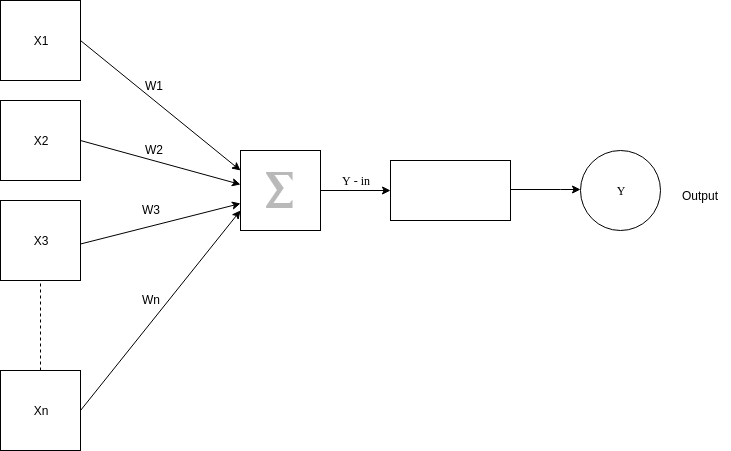
\includegraphics[height=7cm]{Pictures/ann_model.png}
\caption{ANN Model}
\label{}
\end{figure}

For the above general model of artificial neural network, the net input can be calculated as follows −

\[Y_{in} = x_{1}*w_{1} + x_{2}*w_{2} + x_{3}*w_{3} + .....+ X_{n}*w_{n}\]

i.e., net input

\[y_{in} = \sum_{i}^{n} x_{i}*w_{i}\]

The output can be calculated by applying the activation function over the net input.
\[Y = F(Y_{in})\]
Output = function (net input calculated)

Processing of ANN depends upon the following three building blocks −

\begin{itemize}
\item Network Topology
\item Adjustments of Weights or Learning
\item Activation Functions

\end{itemize}

\section{NETWORK TOPOLOGY}
A network topology is the arrangement of a network along with its nodes and connecting lines. According to the topology, ANN can be classified as the following kinds −

\subsection{Feedforword Network}
It is a non-recurrent network having processing units/nodes in layers and all the nodes in a layer are connected with the nodes of the previous layers. The connection has different weights upon them. There is no feedback loop means the signal can only flow in one direction, from input to output. It may be divided into the following two types −

\begin{itemize}
\item \textbf{Single layer feedforward network: } The concept is of feedforward ANN having only one weighted layer. In other words, we can say the input layer is fully connected to the output layer.

\end{itemize}

\begin{figure}[htbp]
\centering
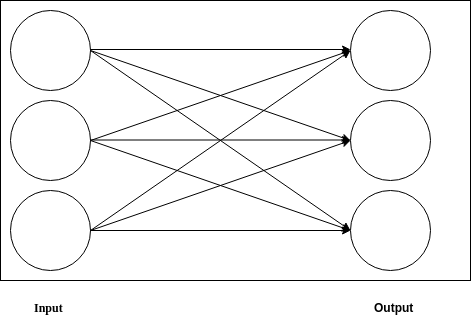
\includegraphics[height=7cm]{Pictures/Single_layer_feedforward_network.png}
\caption{Single Layer Feed Forward Network}
\label{}
\end{figure}

\begin{itemize}
\item \textbf{Multi layer feedforward network: } The concept is of feedforward ANN having more than one weighted layer. As this network has one or more layers between the input and the output layer, it is called hidden layers.


\end{itemize}

\begin{figure}[htbp]
\centering
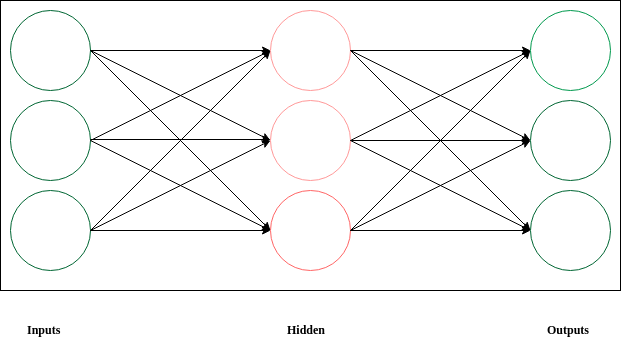
\includegraphics[height=7cm]{Pictures/Multilayer_feedforward_network.png}
\caption{Multilayer Feedforward Network}
\label{}
\end{figure}

\subsection{Feedback Network}
As the name suggests, a feedback network has feedback paths, which means the signal can flow in both directions using loops. This makes it a non-linear dynamic system, which changes continuously until it reaches a state of equilibrium. It may be divided into the following types −

\begin{itemize}
\item \textbf{Recurrent networks} They are feedback networks with closed loops. Following are the two types of recurrent networks.

\item \textbf{Fully recurrent network} It is the simplest neural network architecture because all nodes are connected to all other nodes and each node works as both input and output.

\begin{figure}[htbp]
\centering
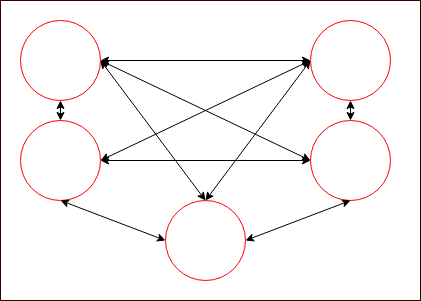
\includegraphics[height=7cm]{Pictures/fully_recurrent_network.png}
\caption{Fully Recurrent Network}
\label{}
\end{figure}

\item \textbf{Jordan network} It is a closed loop network in which the output will go to the input again as feedback as shown in the following diagram.


\begin{figure}[htbp]
\centering
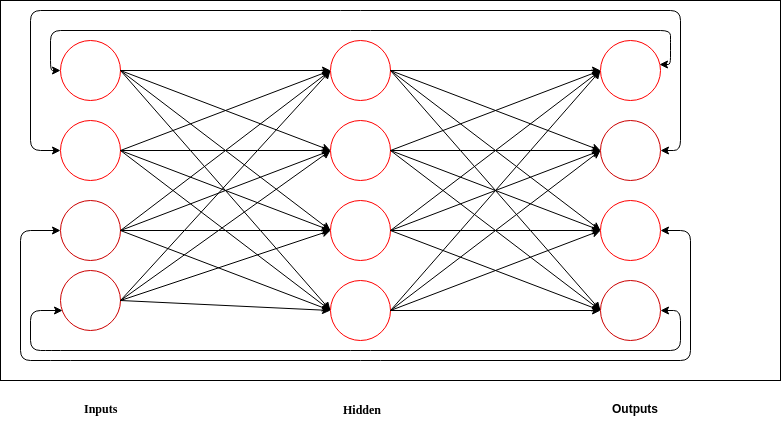
\includegraphics[height=7cm]{Pictures/Jordan_network.png}
\caption{Jordan Network}
\label{}
\end{figure}

\end{itemize}

\section{Adjustments of Weights or Learning}
Learning, in artificial neural network, is the method of modifying the weights of connections between the neurons of a specified network. Learning in ANN can be classified into three categories namely supervised learning, unsupervised learning, and reinforcement learning.
\subsection{Supervised Learning}

As the name suggests, this type of learning is done under the supervision of a teacher. This learning process is dependent.
\paragraph{}
During the training of ANN under supervised learning, the input vector is presented to the network, which will give an output vector. This output vector is compared with the desired output vector. An error signal is generated, if there is a difference between the actual output and the desired output vector. On the basis of this error signal, the weights are adjusted until the actual output is matched with the desired output.

\begin{figure}[htbp]
\centering
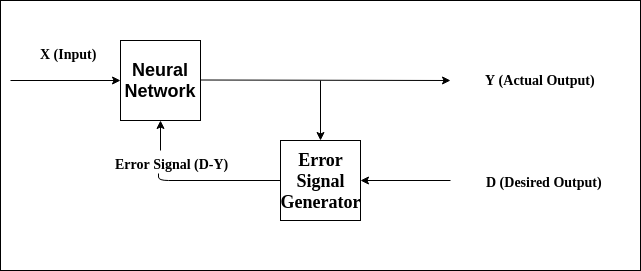
\includegraphics[height=7cm]{Pictures/Supervised_Learning.png}
\caption{Supervised Learning}
\label{}
\end{figure}

\subsection{Unsupervised Learning}
As the name suggests, this type of learning is done without the supervision of a teacher. This learning process is independent.
\paragraph{}
During the training of ANN under unsupervised learning, the input vectors of similar type are combined to form clusters. When a new input pattern is applied, then the neural network gives an output response indicating the class to which the input pattern belongs.
There is no feedback from the environment as to what should be the desired output and if it is correct or incorrect. Hence, in this type of learning, the network itself must discover the patterns and features from the input data, and the relation for the input data over the output.

\begin{figure}[htbp]
\centering
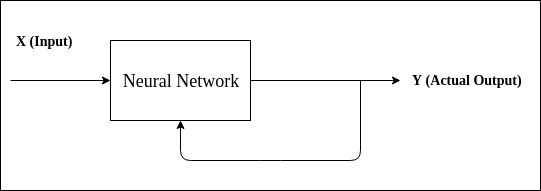
\includegraphics[height=7cm,width = 16cm]{Pictures/Unsupervised_Learning.png}
\caption{Unsupervised Learning}
\label{}
\end{figure}

\subsection{Reinforcement Learning}

As the name suggests, this type of learning is used to reinforce or strengthen the network over some critic information. This learning process is similar to supervised learning, however we might have very less information.
\paragraph{}
During the training of network under reinforcement learning, the network receives some feedback from the environment. This makes it somewhat similar to supervised learning. However, the feedback obtained here is evaluative not instructive, which means there is no teacher as in supervised learning. After receiving the feedback, the network performs adjustments of the weights to get better critic information in future.

\begin{figure}[htbp]
\centering
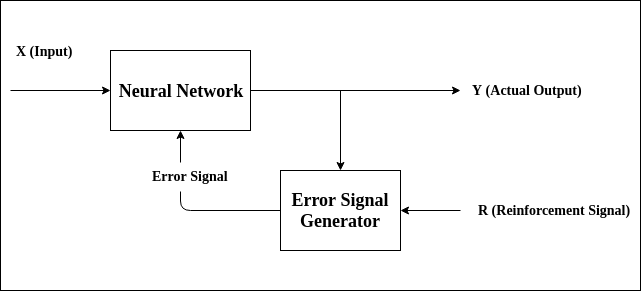
\includegraphics[height=7cm]{Pictures/Reinforcement_Learning.png}
\caption{Reinforcement Learning}
\label{}
\end{figure}


\section{Activation Functions}
It may be defined as the extra force or effort applied over the input to obtain an exact output. In ANN, we can also apply activation functions over the input to get the exact output. Followings are some activation functions of interest −

\subsection{Linear Activation Function}
It is also called the identity function as it performs no input editing. It can be defined as −
\[f(x) = x\]

\subsection{Sigmoid Activation Function}
It is of two type as follows −

\begin{itemize}
\item \textbf{Binary sigmoidal function} This activation function performs input editing between 0 and 1. It is positive in nature. It is always bounded, which means its output cannot be less than 0 and more than 1. It is also strictly increasing in nature, which means more the input higher would be the output. It can be defined as
\[f(x) = \frac{1}{1+e^{-x}}\]

\item \textbf{Bipolar sigmoidal function} This activation function performs input editing between -1 and 1. It can be positive or negative in nature. It is always bounded, which means its output cannot be less than -1 and more than 1. It is also strictly increasing in nature like sigmoid function. It can be defined as\[f(x) = \frac{2}{1+e^{-x}}-1 = \frac{1-e^{x}}{1+e^{x}}\]


\end{itemize}

%\begin{table}[htbp]
%\resizebox{1.1\textwidth}{!}{
%\begin{tabular}{|l|l|l|}
%\hline
%Criteria & BNN & ANN \\ \hline
%Processing & Massively parallel, Slow but superior than ANN & Massively Parallel, Fast but inferior than BNN \\ \hline
% &  &  \\ \hline
% &  &  \\ \hline
% &  &  \\ \hline
% &  &  \\ \hline
%\end{tabular}}
%\end{table}


\section{Learning}
The type of learning we will discuss is commonly called supervised learning or error correction learning. The algorithm that we have used to do this is called Back Propagation of Error signals or in short Backprop. Every iteration of the algorith consists of two pases: 

\subsection{Forward Pass: }
Forward pass every perceptron calculates the weighted linear combination of all its inputs and applies to the result of this summing junction an activation function. The result of the activation function provides the perceptron of its output value.

\subsection{Backward Pass: }
 At the output layer of the network we calculate the error with respect to the desired output value for a certain pattern. This error is propagated backwards through the network enforcing a correction on the weights of all connections in the network. This technique is based on the observation that all perceptrons in the network have a shared  responsibility for the error that has been calculated at the output layer.

\section{Optimization Algorithms Used:}
\subsection{Adagrad: }
Adagrad is an algorithm for gradient-based optimization that does just this: It adapts the learning rate to the parameters, performing smaller updates
(i.e. low learning rates) for parameters associated with frequently occurring features, and larger updates (i.e. high learning rates) for parameters associated with infrequent features. For this reason, it is well-suited for dealing with sparse data.
\paragraph{}
\textbf{Pros: }
\begin{itemize}
\item Well Suited for dealing with sparse data
\item Significantly improves the robustness of SGD
\item Lesser need to manually tune learning rate

\end{itemize}

\paragraph{}
\textbf{Cons: }
\begin{itemize}

\end{itemize}

\begin{itemize}
\item Accumulates squared gradients in denominator. Causes the learning rate to shrink and become infinitesimally small.  

\end{itemize}


\subsection{Adadelta: }
Adadelta is a more robust extension of Adagrad that adapts learning rates based on a moving window of gradient updates, instead of accumulating all past gradients. This way, Adadelta continues learning even when many updates have been done. Compared to Adagrad, in the original version of Adadelta you don't have to set an initial learning rate. In this version, initial learning rate and decay factor can be set, as in most other Keras optimizers.

\paragraph{}

\subsection{Adam: }
Adaptive Moment Estimation (Adam) is another method that computes adaptive learning rates for each parameter. In addition to storing an exponentially decaying average of past squared gradients similar to momentum. Whereas momentum can be seen as a ball running down a slope, Adam behaves like a heavy ball with friction, which thus prefers flat minima in the error surface.
\paragraph{}

\subsection{SGD: }
The word ‘stochastic‘ means a system or a process that is linked with a random probability. Hence, in Stochastic Gradient Descent, a few samples are selected randomly instead of the whole data set for each iteration. In Gradient Descent, there is a term called “batch” which denotes the total number of samples from a dataset that is used for calculating the gradient for each iteration. In typical Gradient Descent optimization, like Batch Gradient Descent, the batch is taken to be the whole dataset. Although, using the whole dataset is really useful for getting to the minima in a less noisy or less random manner, but the problem arises when our datasets get really huge.
Suppose, you have a million samples in your dataset, so if you use a typical Gradient Descent optimization technique, you will have to use all of the one million samples for completing one iteration while performing the Gradient Descent, and it has to be done for every iteration until the minima is reached. Hence, it becomes computationally very expensive to perform.
This problem is solved by Stochastic Gradient Descent. In SGD, it uses only a single sample, i.e., a batch size of one, to perform each iteration. The sample is randomly shuffled and selected for performing the iteration.

\chapter{Environment Setup And Performance Metrices}

\section{Dataset: }
The datasets contains transactions made by credit cards in September 2013 by european cardholders. This dataset presents transactions that occurred in two days, where we have 492 frauds out of 284,807 transactions. The dataset is highly unbalanced, the positive class (frauds) account for 0.172 percent of all transactions.
It contains only numeric input variables which are the result of a PCA transformation. Unfortunately, due to confidentiality issues, we cannot provide the original features and more background information about the data. Features V1, V2, ... V28 are the principal components obtained with PCA, the only features which have not been transformed with PCA are 'Time' and 'Amount'. Feature 'Time' contains the seconds elapsed between each transaction and the first transaction in the dataset. The feature 'Amount' is the transaction Amount, this feature can be used for example-dependant cost-sensitive learning. Feature 'Class' is the response variable and it takes value 1 in case of fraud and 0 otherwise.

\section{Environment: }
\subsection{Jupyter Notebook: }
The Jupyter Notebook is an interactive computing environment that enables users to author notebook documents that include: - Live code - Interactive widgets - Plots - Narrative text - Equations - Images - Video.

\subsubsection{Components: } The Jupyter Notebook combines three components:

\begin{itemize}
\item \textbf{The Notebook Web Application: } An interactive web application for writing and running code interactively and authoring notebook documents.

\item \textbf{Kernals: } Separate processes started by the notebook web application that runs users’ code in a given language and returns output back to the notebook web application. The kernel also handles things like computations for interactive widgets, tab completion and introspection.

\item \textbf{Notebook Documents: } Self-contained documents that contain a representation of all content visible in the notebook web application, including inputs and outputs of the computations, narrative text, equations, images, and rich media representations of objects. Each notebook document has its own kernel.

\end{itemize}

\subsection{Operating System: }
This project is done on Linux Operating Systems.


\section{Confusion Matrix: }
A confusion matrix is a summary of prediction results on a classification problem.
The number of correct and incorrect predictions are summarized with count values and broken down by each class. This is the key to the confusion matrix.
The confusion matrix shows the ways in which your classification model is confused when it makes predictions.
It gives us insight not only into the errors being made by a classifier but more importantly the types of errors that are being made.

\begin{figure}[htbp]
\centering
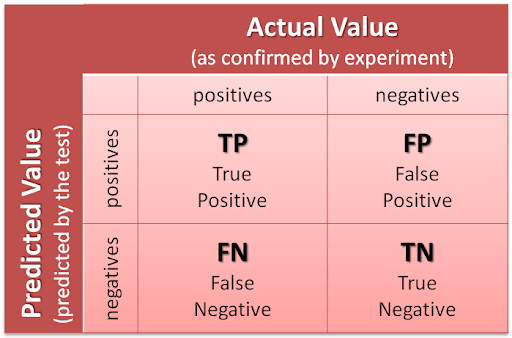
\includegraphics[height=7cm]{Pictures/confusion_matrix.png}
\caption{}
\label{}
\end{figure}

\textbf{Definition of the Terms: }
\begin{itemize}
\item \textbf{True Positive (TP):} Observation is positive, and is predicted to be positive.
\item \textbf{False Negative (FN):} Observation is positive, but is predicted negative.
\item \textbf{True Negative (TN):} Observation is negative, and is predicted to be negative.
\item \textbf{False Positive (FP):} Observation is negative, and is predicted to be positive.
\end{itemize}

\subsection{Classification Rate/Accuracy:}
Classification Rate or Accuracy is given by the relation:
\[Accuracy = \frac{TP + TN}{TP + TN + FP + FN}\]

\subsection{Recall: }
Recall can be defined as the ratio of the total number of correctly classified positive examples divide to the total number of positive examples. High Recall indicates the class is correctly recognized (small number of FN).

Recall is given by the relation:
\[Recall = \frac{TP}{TP + FN}\]


\subsection{Precision: }
To get the value of precision we divide the total number of correctly classified positive examples by the total number of predicted positive examples. High Precision indicates an example labeled as positive is indeed positive (small number of FP).
Precision is given by the relation:

Recall is given by the relation:
\[Recall = \frac{TP}{TP + FP}\]

\begin{itemize}

\item \textbf{High recall, low precision:}
This means that most of the positive examples are correctly recognized (low FN) but there are a lot of false positives.

\item \textbf{Low recall, high precision:}
This shows that we miss a lot of positive examples (high FN) but those we predict as positive are indeed positive (low FP)
\end{itemize}

\subsection{F Measure: }
Since we have two measures (Precision and Recall) it helps to have a measurement that represents both of them. We calculate an F-measure which uses Harmonic Mean in place of Arithmetic Mean as it punishes the extreme values more.
The F-Measure will always be nearer to the smaller value of Precision or Recall.

\[F-measure = \frac{2 * recall * precision}{recall + precision}\]



\section{Performance Metrices: }
% Please add the following required packages to your document preamble:
% \usepackage{multirow}
\begin{table}[htbp]
\begin{tabular}{|l|l|l|l|l|}
\hline
\multicolumn{5}{|c|}{\textbf{Performance Measures}} \\ \hline
\multirow{5}{*}{\textbf{Algorithms}} & \textbf{} & \textbf{Precesion} & \textbf{Recall} & \textbf{F-Score} \\ \cline{2-5} 
 & \textbf{ADAM} & 0.87 & 0.84 & 0.85 \\ \cline{2-5} 
 & \textbf{SGD} & 0.88 & 0.86 & 0.87 \\ \cline{2-5} 
 & \textbf{ADAGARD} & 0.98 & 0.81 & \textbf{0.89} \\ \cline{2-5} 
 & \textbf{ADADELTA} & 0.62 & 0.8 & 0.7 \\ \hline
\end{tabular}
\end{table}


\begin{table}[htbp]
\begin{tabular}{|l|l|}
\hline
 & \textbf{Accuracy} \\ \hline
\textbf{ADAM} & 99.94 \\ \hline
\textbf{SGD} & 99.95 \\ \hline
\textbf{ADAGARD} & \textbf{99.96} \\ \hline
\textbf{ADADELTA} & 99.89 \\ \hline
\end{tabular}
\end{table}

\textbf{Confusion Metrices: }

\begin{figure}[htbp]
\centering
    \subfigure[]{\label{fig:adam}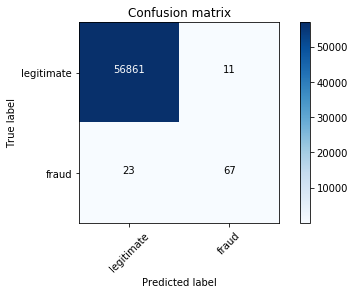
\includegraphics[width=0.49\linewidth]{adam.png}}
    \subfigure[]{\label{fig:sgd}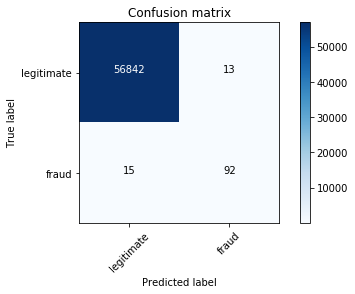
\includegraphics[width=0.49\linewidth]{sgd.png}} 
    \\
    \subfigure[]{\label{fig:adagrad}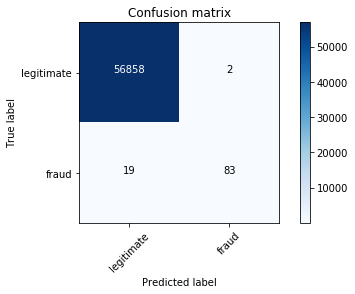
\includegraphics[width=0.49\linewidth]{adagrad.png}}
    \subfigure[]{\label{fig:adadelta}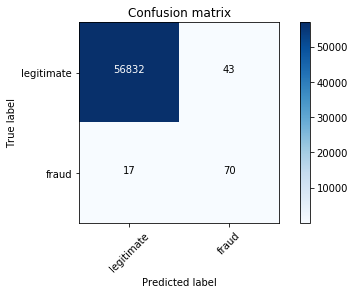
\includegraphics[width=0.49\linewidth]{adadelta.png}} 
  \label{fig:cm}
  \caption{Confusion matrix comparison among \ref{fig:adam} ADAM, \ref{fig:sgd} SGD, \ref{fig:adagrad} ADAGRAD, \ref{fig:adadelta} ADADELTA}
\end{figure}


\begin{figure}[htbp]
\centering
    \subfigure[]{\label{fig:adam_model_accuracy}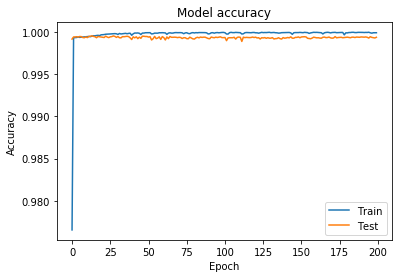
\includegraphics[width=0.49\linewidth]{adam_model_accuracy.png}}
    \subfigure[]{\label{fig:sgd_model_accuracy}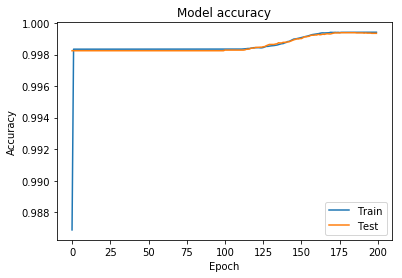
\includegraphics[width=0.49\linewidth]{sgd_model_accuracy.png}} 
    \\
    \subfigure[]{\label{fig:adagrad_model_accuracy}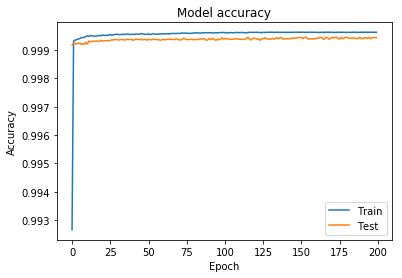
\includegraphics[width=0.49\linewidth]{adagrad_model_accuracy.png}}
    \subfigure[]{\label{fig:adadelta_model_accuracy}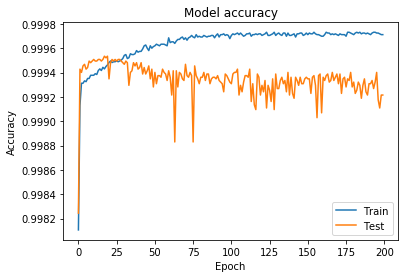
\includegraphics[width=0.49\linewidth]{adadelta_model_accuracy.png}} 
  \label{fig:model accuracy}
  \caption{Model Accuracy Comparison among \ref{fig:adam_model_accuracy} ADAM, \ref{fig:sgd_model_accuracy} SGD, \ref{fig:adagrad_model_accuracy} ADAGRAD, \ref{fig:adadelta_model_accuracy} ADADELTA}
\end{figure}

\begin{figure}[htbp]
\centering
    \subfigure[]{\label{fig:adam_model_loss}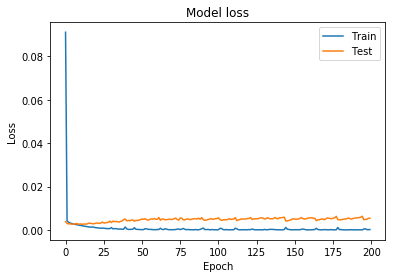
\includegraphics[width=0.49\linewidth]{adam_model_loss.png}}
    \subfigure[]{\label{fig:sgd_model_loss}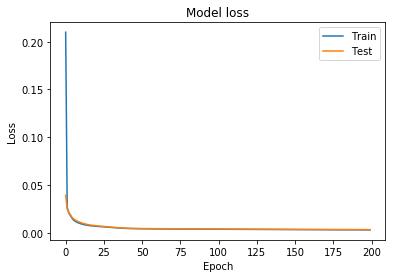
\includegraphics[width=0.49\linewidth]{sgd_model_loss.png}} 
    \\
    \subfigure[]{\label{fig:adagrad_model_loss}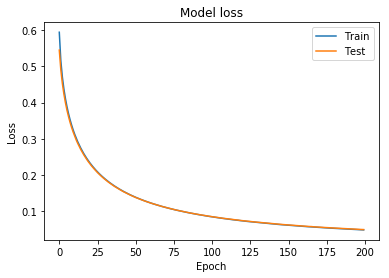
\includegraphics[width=0.49\linewidth]{adagrad_model_loss.png}}
    \subfigure[]{\label{fig:adadelta_model_loss}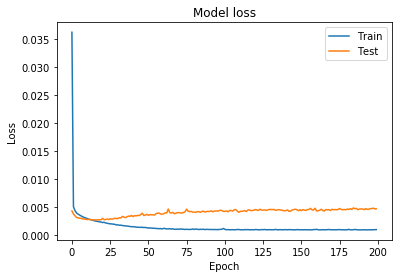
\includegraphics[width=0.49\linewidth]{adadelta_model_loss.png}} 
  \label{model loss}
  \caption{Model Loss Comparison among \ref{fig:adam_model_loss} ADAM, \ref{fig:sgd_model_loss} SGD, \ref{fig:adagrad_model_loss} ADAGRAD, \ref{fig:adadelta_model_loss} ADADELTA}
\end{figure}


\chapter{Result Discussion}
\section{Performance Comparisons}

\begin{figure}[htbp]
\centering
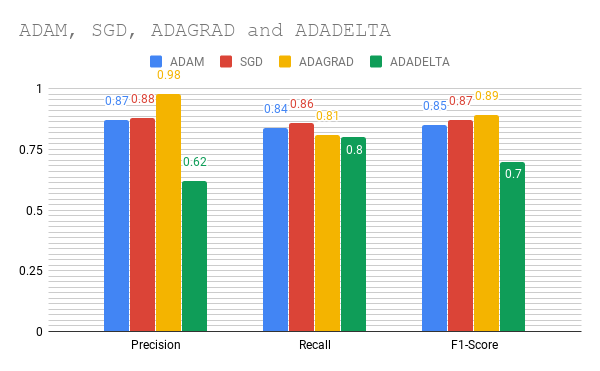
\includegraphics[height=7cm]{Pictures/ADAM_SGD_ADAGRAD_and_ADADELTA_graph.png}
\caption{Precision, Recall and F-score comparison among ADAM, SGD, ADAGRAD, ADADELTA}
\label{}
\end{figure}

As it is given in the above graph that ADAGRAD is having the heighest F-score so this optimizer algorithm is giving the best performance among these four algorithms. After this SGD, ADAM, ADADELTA are having better performances in decreasing order. 

\begin{figure}[htbp]
\label{fig:accuracy}
\centering
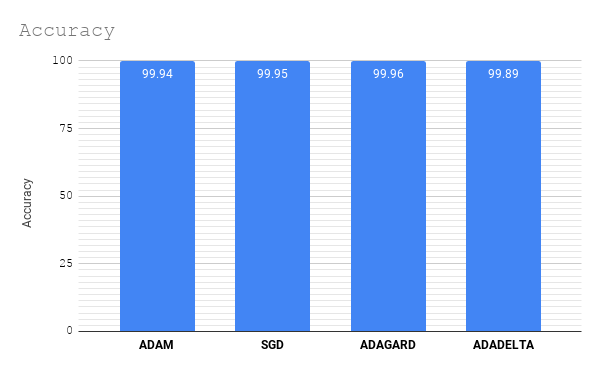
\includegraphics[height=7cm]{Pictures/Accuracy_chart.png}
\caption{Accuracy Comparison among ADAM, SGD, ADAGRAD, ADADELTA}
%\label{}
\end{figure}

%\begin{figure}[]
%\centering
%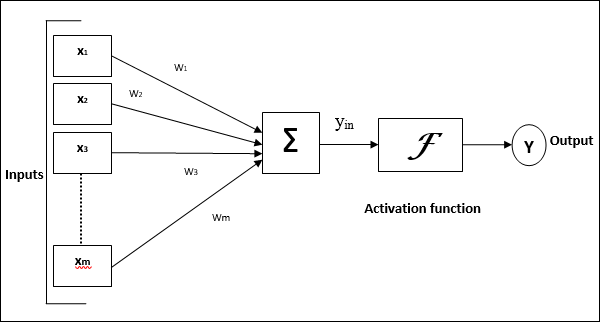
\includegraphics[height=7cm]{Pictures/temp.png}
%\caption{Splitting of the input space (X1 x X2) by M5' model tree algorithm}
%\label{fig5}
%\end{figure}

%\begin{figure}[]
%\centering
%\includegraphics[height=7cm]{Pictures/Neuron3.png}
%\caption{Splitting of the input space (X1 x X2) by %M5' model tree algorithm}
%\label{fig5}
%\end{figure}

%\begin{figure}[]
%\centering
%\includegraphics[height=7cm]{Pictures/neural-%network.png}
%\caption{Splitting of the input space (X1 x X2) by %M5' model tree algorithm}
%\label{fig5}
%\end{figure}


\end{document}

